\documentclass[11pt]{article}
\usepackage{amssymb}
\usepackage{amsthm}
\usepackage{amsmath}
\usepackage{listings}
\usepackage{color}
\usepackage{graphicx}

\lstdefinestyle{matlab-style}{
language=Matlab,
basicstyle=\scriptsize\ttfamily,
tabsize=2,
rulecolor=,
language=matlab,
basicstyle=\scriptsize,
aboveskip={1.5\baselineskip},
columns=fullflexible,
showstringspaces=false,
extendedchars=true,
breaklines=true,
prebreak = \raisebox{0ex}[0ex][0ex]{\ensuremath{\hookleftarrow}},
frame=single,
showtabs=false,
showspaces=false,
showstringspaces=false,
identifierstyle=\ttfamily,
keywordstyle=\color[rgb]{0,0,1},
commentstyle=\color[rgb]{0.133,0.545,0.133},
stringstyle=\color[rgb]{0.627,0.126,0.941},
keepspaces=true,
numbers=left,
numbersep=5pt,
numberstyle=\tiny\color[rgb]{0.5,0.5,0.5},
stepnumber=1
}

\title{Design of an optimal heat exchanger\\MANE 6963 - Project 1}
\author{Unique ID goes here}
\date{}

\begin{document}

\maketitle

\section{Introduction}

In this report, we investigate the optimal design of a heat exchanger that
heats air using hot water.

\begin{figure}[htb]
\centering
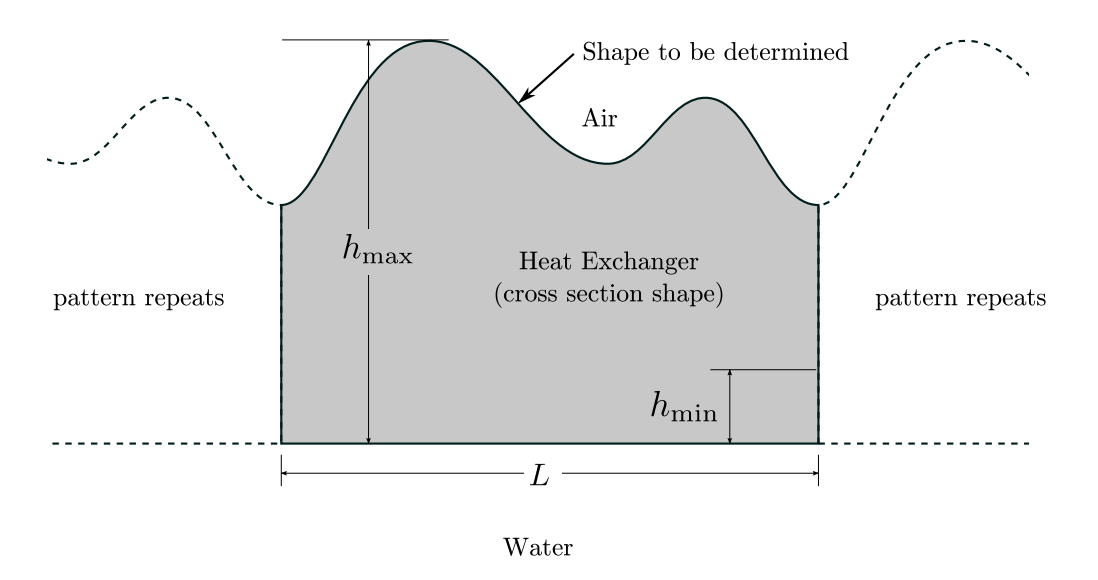
\includegraphics[scale=0.5]{exchanger}
\caption{Geometry of the heat exchanger design problem}
\end{figure}

\section{Executive summary}

\section{Analysis methods}

The transfer of heat from the water to the air is modeled with the
two-dimensional steady heat equation.
\begin{align*}
- \nabla \cdot (\kappa \nabla T) &= 0, \quad \forall x \in \Omega, \\
T(x,y=0) &= T_{\text{water}}, \\
T(x,y=h(x)) &= T_{\text{air}}, \\
T(x,y) &= T(x+L,y).
\end{align*}
Dirichlet boundary conditions are set at the bottom and top
surfaces of the heat exchanger geometry, such that the temperature
at the bottom surface is prescribed to  

The material of the heat conductor is assumed to be isotropic, that is
the thermal conductivity coefficient $\kappa$ has no spatial dependence.

\section{Geometry parameterization}

The geometry is parameterized such that

\[
h(x,\boldsymbol{p}) = p_1 + \sum_{k=0}^{N_p} p_k 
\left[ \sin \left( \frac{2 \pi (k-1) x}{L} \right) \right]^2
\]


\section{Optimization methods}

\section{Results}

\begin{center}
\scriptsize
\begin{verbatim}
                                                           Norm of First-order
 Iter F-count            f(x) Feasibility  Steplength        step  optimality
    0       7    1.904069e-04   1.886e+00                           3.503e-04
    1      14    1.084683e-04   2.249e-09   1.000e+00   1.263e+00   8.121e-01
    2      21    1.025917e-04   0.000e+00   1.000e+00   1.796e-03   2.054e-03
    3      28    9.434870e-05   0.000e+00   1.000e+00   3.731e-03   1.889e-03
    4      35    9.081085e-05   0.000e+00   1.000e+00   2.909e-03   1.727e-03
    5      42    7.626375e-05   0.000e+00   1.000e+00   1.074e-02   2.329e-03
    6      49    5.690875e-05   0.000e+00   1.000e+00   3.370e-02   1.860e-03
    7      56    5.299726e-05   0.000e+00   1.000e+00   7.231e-03   4.072e-04
    8      63    4.866073e-05   0.000e+00   1.000e+00   5.966e-03   7.180e-04
    9      70    3.709187e-05   0.000e+00   1.000e+00   1.277e-02   1.257e-03
   10      77    3.689727e-05   0.000e+00   1.000e+00   5.197e-04   3.276e-04
   11      84    3.591001e-05   1.908e-17   1.000e+00   2.604e-03   3.346e-04
   12      91    3.505216e-05   1.214e-17   1.000e+00   2.138e-03   3.801e-04
   13      98    3.404131e-05   4.805e-13   1.000e+00   2.385e-03   3.642e-04
   14     105    3.404131e-05   2.082e-17   1.000e+00   7.822e-13   4.682e-10
\end{verbatim}
\end{center}

\newpage

\section{Appendix: code listings}

\lstinputlisting[
  style=matlab-style,
  caption=SurfaceHeight.m]{SurfaceHeight.m}

\newpage

\lstinputlisting[ 
  style=matlab-style,
  caption=NonlinearConstraints.m]{NonlinearConstraints.m}

\newpage

\lstinputlisting[
  style=matlab-style,
  caption=MaxFluxDriver.m]{MaxFluxDriver.m}

\end{document}
